\section{Implementierung des Backends auf Basis von Alfresco} \label{Implementierung Backend}
F\"ur das Backend eignet sich der Analyse aus Kapitel \ref{Technologievergleich} folgend am besten Alfresco. In den nun folgenden Abschnitten geht es um die Implementierung des Metadatenmodells aus Kapitel \ref{Erstellung eines Datenkonzepts} in Alfresco. Hierf\"ur wird zum Einen die Installation und die Arbeitsweise erl\"autert und zum Anderen wird im Hauptteil auf die Implementierung des Datenmodells in Alfresco eingegangen.

\subsection{Installation}
Die Installation von Alfresco ist denkbar einfach und unter Windows, sowie unter Linux m\"oglich. F\"ur den Download der Community Edition muss man sich mit einer g\"ultigen E-Mail-Adresse bei Alfresco anmelden\footnote{https://www.alfresco.com/de/products/community/download}. 

Die Anmeldung hat den Vorteil, dass der Nutzer zu Webinars und anderen neuen Dingen rund um Alfresco immer auf dem Laufenden ist.
Die kostenpflichtige Variante von Alfresco bietet zus\"atzliche technische Unterst\"utzung und einige Enterprise Features, welche jedoch f\"ur diese Arbeit nicht ben\"otigt werden. \cite{Wiki_Alfresco}

Nach dem Download f\"uhrt unter Linux ein Skript die Installation durch. Hierbei wird der Nutzer ausf\"uhrlich \"uber alle durgef\"uhrten Schritte informiert. Der Nutzer muss w\"ahrend der Installation ein Passwort f\"ur das Administrator-Konto angeben.\cite{Alfresco_und_Liferay}

Ist die Installation abgeschlossen und der Server gestartet, kann Alfresco im Browser lokal unter \url{http://127.0.0.1:8080/share/page/} aufgerufen werden.

War die Anmeldung erfolgreich, gelangt der Nutzer auf das "`Administrator Dashboard"', welches in Abbildung \ref{Alfresco Dashboard} im Abschnitt \ref{Alfresco} zu sehen ist.

\subsection{Metadatenmodell in Alfresco} \label{Metadatenmodell von Alfresco}
Um ein eigenes Metadatenmodell in Alfresco einf\"ugen zu k\"onnen, muss es mittels XML beschrieben werden. Unter \texttt{ALFRESCO\_HOME} wird im Folgenden das Home-Verzeichnis des Alfresco-Servers zu verstehen sein. 

In Abbildung \ref{Alfresco Content-Modell} ist das Content-Modell von Alfresco in UML dargestellt. Das Hauptelement Klasse (Class) beschreibt den Aufbau eines Content-Modells und enth\"alt Aspekte (Aspect) und Typen (Type) welche ganz oben im Diagramm zu sehen sind. \cite{Professional_Alfresco}

Klassen im Content-Modell k\"onnen ihre Eigenschaften, das hei\ss{}t ihre Aspekte und Typen, an Unterklassen vererben. In Alfresco ist nur eine einfache und keie Mehrfachvererbung zul\"assig.

Eine Klasse kann Assoziationen auf andere Klassen (Peer Association) oder Objekte (Property) enthalten. Eine Assoziation auf eine andere Klasse ist unter Alfresco jedoch nur zul\"assig, wenn schon ein Content (Instanz der Klasse) der jeweiligen Klasse existiert, andernfalls muss er vorher angelegt werden. Objekte oder auch Attribute k\"onnen aus einem Constraint oder einem einfachen Datentyp (Data Type) bestehen.

Um das Metadatenmodell, wie in Kapitel \ref{Erstellung eines Datenkonzepts} beschrieben, umsetzen zu k\"onnen, m\"ussten Datentypen auch wieder Klassen enthalten k\"onnen (Komposition). Dies ist jedoch unter keinem der beschriebenen \ac{ECM}-Tools m\"oglich. Jedoch bietet Alfresco den besten Ansatz, weshalb das Datenmodell nun noch einmal f\"ur Alfresco angepasst werden muss. Wie genau das Metadatenmodell angepasst wurde, ist im Abschnitt \ref{Ver\"andertes Datenmodell f\"ur Alfresco} genauer erl\"autert.

Unter Alfresco kann eine Klasse mehrere Typen enthalten, ein Typ kann zum Beispiel ein Bild, ein Gesetz oder \"ahnliches sein. Jeder Typ kann Attribute beinhalten, welche fest mit ihm verbunden sind. Wird eine PDF-Datei in Alfresco also zu einem "`Gesetz"' also zu ein Dokument mit dem Datentyp \texttt{Gesetz} umgewandelt, enth\"alt es unweigerlich nach der \"Anderung alle Attribute, welche direkt im Typ beschrieben und verankert sind.

Ein Aspekt kann frei definiert und zu einem beliebingen Typ hinzuf\"ugt werden. M\"ochte ein Nutzer also die Attribute von \ac{INSPIRE} hinzuf\"ugen, so reicht es, wenn er den entsprechenden Aspekt zu dem gew\"unschten Dokument hinzuf\"ugt. Die jeweiligen Datentypen m\"ussen hierbei als Aspekt definiert sein.

\begin{figure}[!ht]
\centering
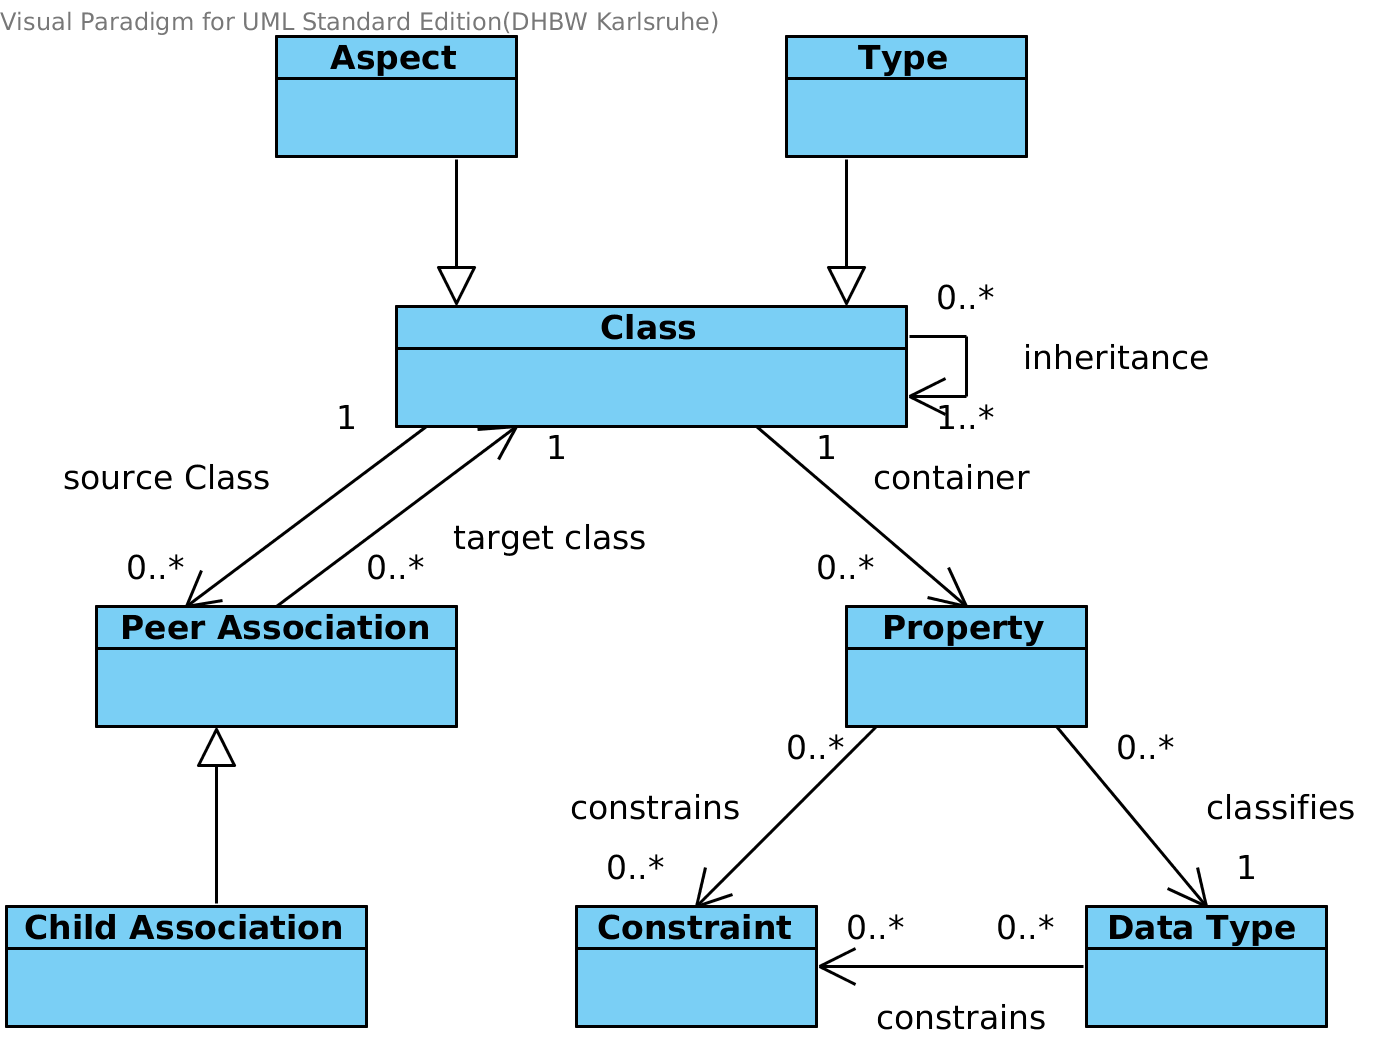
\includegraphics[width=10cm]{Bilder/Alfresco_Contentmodel.png}
\caption{Content-Modell in Alfresco}
\label{Alfresco Content-Modell}
\centering
\end{figure}

\subsection{Ver\"andertes Datenmodell f\"ur Alfresco}\label{Ver\"andertes Datenmodell f\"ur Alfresco}
Wie im Abschnitt \ref{Metadatenmodell von Alfresco} schon ausf\"uhrlich beschrieben, ist es nicht m\"oglich, die zuvor im Kapitel \ref{Erstellung eines Datenkonzepts} erstellte Metadatenstruktur umzusetzen. Daher wird nun beschrieben, wie das Datenmodell f\"ur Alfresco angepasst werden kann.

Da Alfresco den "`Dublin Core"'-Standard bereits implementiert hat, kann dieser direkt genutzt werden. Auch die Datensammlung \texttt{Datei} entf\"allt, da die entsprechenden Daten automatisch bei jeder hochgeladenen Datei von Alfresco ausgelesen und erstellt werden. 

Die im Abschnitt \ref{FADO Metadaten} gezeigten Datensammlungen werden nun zu Datentypen oder Aspekten, welche das jeweilige Dokument beschreiben. Alle farbig hinterlegten Attribute stellen Aspekte dar, die von anderen Klassen aus Alfresco \"ubernommen wurden.
Packages stellen in diesem Diagramm Klassen dar. Die UML-Klassen stellen Aspekte oder Typen dar. Worum es sich genau handelt, steht jeweils auch an den Datensammlungen. 

Alle in den folgenden Abschnitten nicht aufgef\"uhrten Datensammlungen sind direkt in den Aspekten untergebracht, da Alfresco keine Klassen oder Typen als Attribute zul\"asst.

\subsubsection{Die Datentypen}\label{Die Datentypen}
Die in den Abschnitten \ref{FADO Metadaten} bis \ref{ICT-ENSURE Metadaten} gezeigten Grunddatentypen bleiben im angepassten Modell weitestgehend identisch. Da unter Alfresco eine Datei nur von genau einem Datentyp sein kann, wurde die Datensammlung \texttt{FADO Metadaten} den anderen \ac{FADO}-Sammlungen \"ubergeordnet, wie in Abbildung \ref{Fado Datentypen f\"ur Alfresco} zu sehen ist. Der Typ \texttt{Fado Metadaten} findet sich nun in der Klasse \texttt{Fado}, welche wiederum die Oberklasse f\"ur die Typen \texttt{FADO Urteil}, \texttt{Forschungsvorhaben} und \texttt{Bibliografische Angaben} bildet.

\begin{figure}[!ht]
\centering
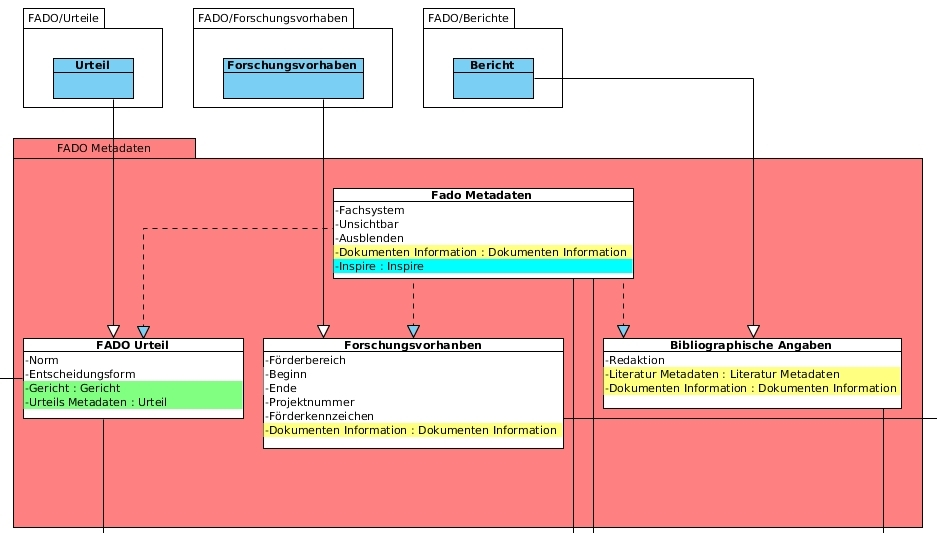
\includegraphics[width=16cm]{Bilder/AlfrescoModell/Fado-Datentypen.jpg}
\caption{FADO Datentypen f\"ur Alfresco}
\label{Fado Datentypen f\"ur Alfresco}
\centering
\end{figure}

Die Datentypen \texttt{DRS-Metadaten} und \texttt{Bildarchiv Metadaten} sind im Grunde gleich geblieben. Hier haben sich nur geringf\"ugige \"Anderungen ergeben, da die Datensammlungen wieder zusammengefasst worden sind. Die beiden Datensammlungen \texttt{Artikel Metadaten} und \texttt{Konferenz} sind zusammengefasst worden und nun im Typ \texttt{Artikel Metadaten} zu finden.
Die eben beschriebenen \"Anderungen sind in den Abbildungen \ref{Bildarchiv und ICT-ENSURE Datentypen f\"ur Alfresco} und \ref{DRS Datentyp f\"ur Alfresco} zu sehen.

\begin{figure}[!ht]
\centering
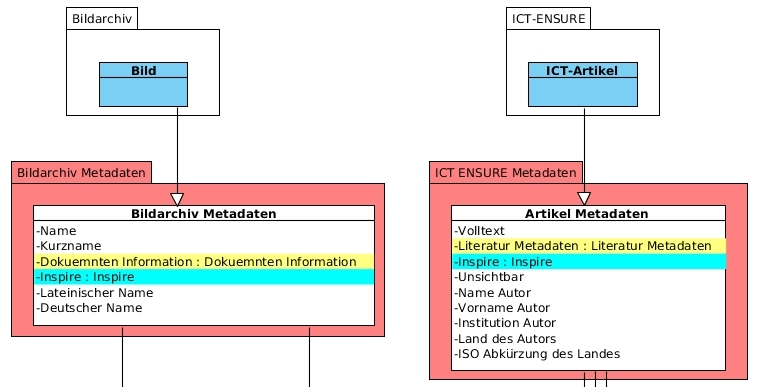
\includegraphics[width=12cm]{Bilder/AlfrescoModell/Bildarchiv-und-ICT-Datentypen.jpg}
\caption{Bildarchiv und ICT-ENSURE Datentypen f\"ur Alfresco}
\label{Bildarchiv und ICT-ENSURE Datentypen f\"ur Alfresco}
\centering
\end{figure}

Im Abschnitt \ref{Die Klasse Gerichtbarkeit} wird noch einmal genauer erw\"ahnt, warum die Attribute \texttt{Fundstelle}, \texttt{Datum Rechtsvorschriften} und \texttt{Ablage} nicht mehr existieren.

\begin{figure}[!ht]
\centering
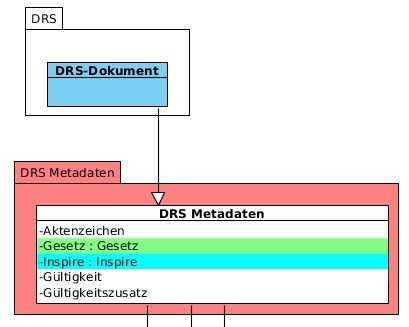
\includegraphics[width=6cm]{Bilder/AlfrescoModell/DRS-Datentypen.jpg}
\caption{DRS Datentyp f\"ur Alfresco}
\label{DRS Datentyp f\"ur Alfresco}
\centering
\end{figure}

\FloatBarrier
\subsubsection{Die Klasse Gerichtbarkeit}\label{Die Klasse Gerichtbarkeit}
Das Package \texttt{Gerichtbarkeit} beschreibt eine Klasse, welche drei Aspekte beinhaltet. Diese Aspekte sind \texttt{Gesetz}, welcher die Datensammlungen \texttt{Fundstelle}, \texttt{Datum der Rechtsvorschriften} und \texttt{Ablage} zusammengefasst, \texttt{Urtei} und \texttt{Gericht}. 

Die Datensammlung \texttt{Gericht} geht ohne Ver\"anderung in einen Aspekt \"uber und wird im Typ \texttt{FADO Urteil} verwendet. Die Sammlung \texttt{Urteil} musste etwas abge\"andert werden. Die Verweise auf das Vorgericht und das Nachgericht wurden aufgeschl\"usselt, da Alfresco bekanntlich keine Klassen als Attribute unterst\"utzt.

In Abbildung \ref{Klasse Gerichtbarkeit} ist die Klasse \texttt{Gerichtbarkeit} noch einmal dargestellt. Zu beachten ist, dass das Package hier f\"ur eine gesamte Klasse steht und die eigentlichen Klassen nur Aspekte darstellen.

\begin{figure}[!ht]
\centering
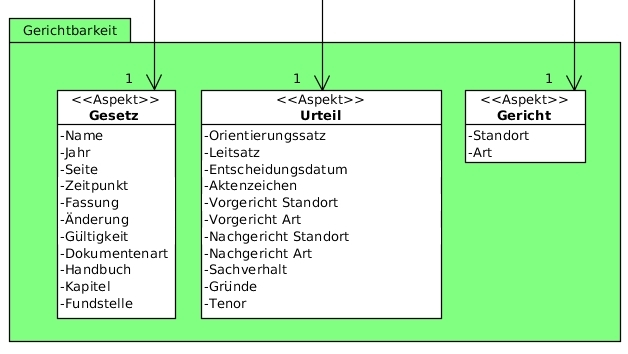
\includegraphics[width=11cm]{Bilder/AlfrescoModell/Gerichtbarkeit.jpg}
\caption{Die Klasse Gerichtbarkeit}
\label{Klasse Gerichtbarkeit}
\centering
\end{figure}

\FloatBarrier
\subsubsection{Die Klasse Standard Aspekte}\label{Die Klasse Standard Aspekte}
Das Package \texttt{Standard Aspekte}, ist wieder eine Metadaten-Klasse von Alfresco, welche den Aspekt \texttt{Inspire} enth\"alt. Durch die \"Anderungen am Datenmodell wurden die Attribute, welche sich in den verweisten Datensammlungen befunden haben, nun direkt in der Datensammlung \texttt{Inspire} untergebracht, welche nun ein Aspekt ist. 

Die Abbildung \ref{Klasse Standard Aspekte} zeigt noch einmal den Aspekt \texttt{Inspire}, welcher sich in der Klasse (dem Package) \texttt{Standard Aspekte} befindet.

\begin{figure}[!ht]
\centering
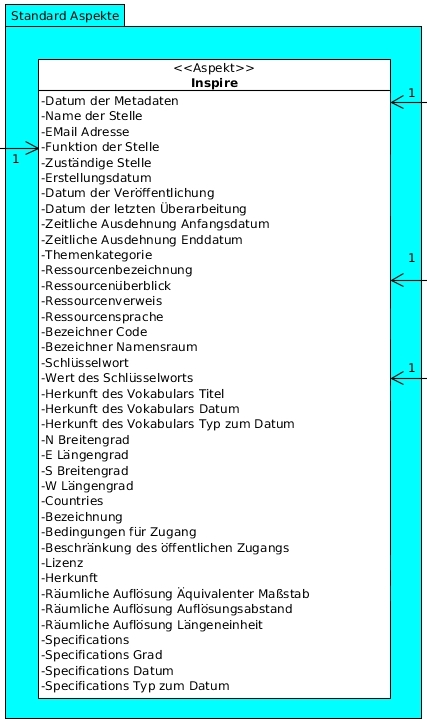
\includegraphics[width=8cm]{Bilder/AlfrescoModell/Standard-Aspekte.jpg}
\caption{Die Klasse Standard Aspekte}
\label{Klasse Standard Aspekte}
\centering
\end{figure}

\FloatBarrier
\subsubsection{Die Klasse Bibliografische Aspekte} \label{Die Klasse Bibliografische Aspekte}
In Abbildung \ref{Klasse Bibligrafische Aspekte} ist die Klasse \texttt{Bibliografische Aspekte} zu sehen, welche die beiden Aspekte \texttt{Dokumenten Information} und \texttt{Literatur Metadaten} enth\"alt.

Beim Aspekt \texttt{Dokumenten Information} ergaben sich keine \"Anderungen, au\ss{}er dass das Attribut "`Stand"' nun eigenst\"andig ist und nicht mehr auf ein Datum verweist. Der Aspekt \texttt{Literatur Metadaten} enth\"alt nun die Attribute der Datensammlungen \texttt{Kapitel} und \texttt{Publikations ID}.

\begin{figure}[!ht]
\centering
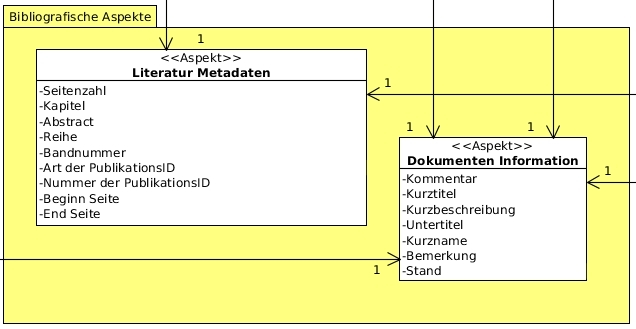
\includegraphics[width=10cm]{Bilder/AlfrescoModell/Bibliografische-Aspekte.jpg}
\caption{Die Klasse Standard Aspekte}
\label{Klasse Bibligrafische Aspekte}
\centering
\end{figure}

\FloatBarrier
\subsection{Implementierung einer Datensammlung}
Eine Datensammlung in Alfresco wird im Verzeichnis \texttt{ALFRESCO\_HOME/tomcat/shared/classes
/alfresco/extensions} abgelegt.
Wie ein Datenmodell in Alfresco implementiert wird, ist anhand der Datensammlung \texttt{Bildarchiv Metadaten} gezeigt, welche im Listing \ref{Bildarchiv-Metadaten Listing} weiter unten zu sehen ist.

Mit dem Tag "`model"' wird ein Datenmodell in Alfresco beschrieben, alle weiteren Einstellungen werden innerhalb dieses Tags vollzogen. Der Name des Modells wird durch das Prefix und die Namespace-URI gebildet.

Die Tags "`description"', "`author"' und "`version"' geben grundlegende Informationen \"uber das entsprechende Modell und wer daf\"ur verantwortlich ist.

Innerhalb des Tags "`imports"' werden Datenmodelle importiert, welche in dem Modell entsprechend verwendet werden. Grunds\"atzlich werden die Modelle \texttt{http://www.alfresco.org/model/ dictionary/1.0} und \texttt{http://www.alfresco.org/model/content/1.0} immer importiert, da sie den Grundstock eines jeden Modells bilden.

Zus\"atzlich werden die beiden Modelle \texttt{Bibliografische-Aspekte} und \texttt{Standard-Metadaten} importiert (siehe Abschnitt \ref{Die Klasse Bibliografische Aspekte} und \ref{Die Klasse Standard Aspekte}), da ihre Aspekte innerhalb des Modells verwendet werden. Hierzu sp\"ater mehr.

Der Tag "`namespaces"' definiert den Namensraum, in welchem das Datenmodell verwendet wird. Mit "`namespace"' wird der spezifische Namensraum zum einen durch eine URI, zum anderen durch ein ein Pr\"afix festgelegt. Das Pr\"afix ist eine Abk\"urzung, um nicht immer die komplette URI angeben zu m\"ussen. Die URI wiederum gibt an, wo das Datenmodell abgelegt wird, beziehungsweise zu finden ist.

"`constraints"' ist ein Tag, welcher mehrere Constraints beinhalten kann, wobei ein Constraint einen regul\"aren Ausdruck (Regex) enth\"alt und eine Zeichenfolge genauer beschreibt. Wird ein entsprechendes Constraint auf ein Textfeld angewendet, so wird beim Speichern des Dokuments von Alfresco \"uberpr\"uft, ob das jeweilige Attribut der Vorgabe des Constraints entspricht. Im Datenmodell \texttt{Bibliografische-Aspekte} gibt es keine Constraints, weshalb der entsprechende Tag leer ist.

Zus\"atzlich k\"onnen mit Constraints auch Auswahllisten realisiert werden. Hierbei werden im Constraint alle m\"oglichen Eintr\"age vorgegeben, welche sp\"ater zu Auswahl stehen sollen.

Innerhalb des Tags "`types"' k\"onnen mehrere Dokumenten-Typen spezifiziert werden. Jeder einzelne Typ ist grunds\"atzlich so aufgebaut wie der im Beispielcode in Listing \ref{Bildarchiv-Metadaten Listing} unten. Der Typ hat einen Namen, welcher mit dem Pr\"afix des jeweiligen Namensraums beginnt. 

Im Tag "`title"' wird der Standardtitel angegeben, welcher angezeigt wird, sollte keine I18N-\"Ubersetzung vorliegen. Die \"Ubersetzung wird sp\"ater noch genauer erkl\"art.

Sollte "`parent"' keine eigene Klasse sein, so steht hier standardm\"a\ss{}ig \texttt{cm:content}, welches die Standard-Oberklasse von Alfresco ist.

Unter dem Tag "`properties"' sind alle Attribute zu finden, welche der jeweilige Typ enth\"alt. Innerhalb einer "`property"' wird wiederum der Name des Attributs angegeben. Im Tag "`title"' findet sich der Standardtitel. "`type"' gibt an, von welchem Typ das Attribut ist. Eine genaue Auflistung alles Datentypen von Alfresco ist in der Dokumentation\footnote{\url{http://docs.alfresco.com/4.0/concepts/metadata-model-props.html}} zu finden. Im Tag "`constraints"' k\"onnen Verweise zu einzelnen Constraints des Datenmodells oder aber zu Constraints anderer Datenmodelle angegeben werden. 

\"Uber den Tag "`mandatory-aspects"' k\"onnen Aspekte angegeben werden, welche der Dokumententyp zwingend beinhalten muss. Im Beispiel w\"aren das die Aspekte \texttt{Inspire} und \texttt{Dokumenten-Information}. Beide Aspekte sind auch im Datenmodell in Abbildung \ref{Bildarchiv und ICT-ENSURE Datentypen f\"ur Alfresco} zu sehen.

"`aspects"' kann mehrere Aspekte der jeweiligen Klasse enthalten. Diese Aspekte k\"onnen dann innerhalb der Klasse, sowie klassen\"ubergreifend eingesetzt werden. Grunds\"atzlich sind die Beschreibungen von Aspekten genau wie die von Typen aufgebaut und beinhalten die selben Tags. Einzige Ausnahme ist der Tag "`parent"', da ein Aspekt keinen \"ubergeordneten Datentyp beinhaltet. Im Beispiel sind keine Aspekte vorhanden, da das Datenmodell dies f\"ur die Klasse \texttt{Bildarchiv Metadaten} nicht vorsieht. 

\lstinputlisting[language=xml, caption=Inhalt der Datei Bildarchiv-Metadaten.xml, label=Bildarchiv-Metadaten Listing]{Code/Bildarchiv-Metadaten.xml}

\subsubsection{Das Modell in Alfresco einbinden} \label{Das Modell in Alfresco einbinden}
Um das Datenmodell nun in Alfresco bekannt zu machen, muss eine Context-Datei erstellt werden, welche das Java-Bean beschreibt. Die Context-Datei endet auf "`-context.xml"' und muss im Ordner \texttt{ALFRESCO\_HOME/tomcat/shared/classes/alfresco/extensions} abgelegt werden.

Im Listing \ref{Bildarchiv-Metadaten-context Listing} ist die Context-Datei zu sehen, welche beschreibt wo genau die Klasse zu finden ist.
Das "`bean"' hat zum Einen eine \texttt{id} und ein \texttt{parent}. Zum Anderen ein Attribut, auf welchen Beans es bassiert, was im Attribut \texttt{depends-on} beschrieben ist. Im Beispiel sind das die beiden verwendeten Klassen welche auch importiert werden (siehe Listing \ref{Bildarchiv-Metadaten Listing}).

Unter dem Tag "`property"' wird der Speicherort unserer Modell-Datei angeben.

\lstinputlisting[language=xml, caption=Inhalt der Datei Bildarchiv-Metadaten-context.xml, label=Bildarchiv-Metadaten-context Listing]{Code/Bildarchiv-Metadaten-context.xml}

Sind beide Dateien korrekt und an der richtigen Stelle muss Alfresco neu gestartet werden um das Modell aufzunehmen.

\subsubsection{\"Ubersetzungen in Alfresco}
Um Mehrsprachigkeit in Alfresco zu realisieren verwendet das System Property-Dateien, in welchen die verschiedenen \"Ubersetzungen zu finden sind. Die Property-Dateien m\"ussen unter \texttt{ALFRESCO\_HOME/tomcat/shared/classes/alfresco/messages} abgelegt werden.

Die Dateien k\"onnen beliebig benannt werden, m\"ussen jedoch das ISO-Sprachk\"urzel am Namensende enthalten. Eine deutsche \"Ubersetzung w\"urde dann zum Beispiel in der Datei \texttt{I18N\_de\_DE.properties} und eine US-Amerikanische unter \texttt{I18N\_en\_US.properties} zu finden sein. Alfresco nutzt die �bersetzungen dann automatisch anhand der eingestellten Systemsprache.

Die Datei beinhalten pro Zeile ein Schl\"ussel-Wert-Paar, welches eine \"Ubersetzung f\"ur genau einen String darstellt.
Im Listing \ref{I18NDatei Listing} ist nur ein Ausschnitt der Datei \texttt{I18N\_de\_DE.properties} zu sehen, um das System zu verdeutlichen.

In den Property-Dateien werden Strings f\"ur Typen mit einem Schl\"ussel \texttt{type.<Namespace>\_<Typname>} bezeichnent. Aspekte werden \"ahnlich wie auch Typen bezeichnent und zwar mit \texttt{aspect.<Namespace>\_<Aspektname>}. Andere Keys, wie zum Beispiel die Keys f\"ur Hilfetexte, k\"onnen frei gew\"ahlt werden.

\lstinputlisting[caption=Ausschnitt des Inhalts der \"Ubersetzungsdatei I18N\_de\_DE.properties, label=I18NDatei Listing]{Code/I18N_de_DE.properties}

\subsection{Modell und \"Ubersetzungen in Alfresco anzeigen}
Nach dem in den vorherigen Abschnitten gezeigt wurde, wie eine Datenmodell f\"ur Alfresco erstellt und eingebunden wird, muss nun noch gekl\"art werden, wie sich \"Ubersetzungen und Datenmodell in Alfresco anzeigen lassen.

\subsubsection{Das Datenmodell anzeigen}\label{Das Datenmodell anzeigen}
Um ein Datenmodell in Alfresco mit all seinen Metadaten in der Pr\"asentation und in den Formularen anzuzeigen, reicht es nicht aus, nur das Bean zu erstellen. Zus\"atzlich muss auch angegeben werden, welche Attribute Alfresco wie darstellen soll. Die Darstellung wird in der Datei \texttt{share-config-custom.xml} beschrieben, welche sich im Verzeichnis \texttt{ALFRESCO\_HOME/tomcat/shared/classes/alfresco/web-extensions} befindet.

Da diese Config-Datei sehr lang werden kann, werden im Folgenden immer nur Ausschnitte gezeigt.

Innerhalb des Tags "`alfresco-config"' ist der im Listing \ref{Config Datenmodell} gezeigte Abschnitt zu finden, welcher jedoch hier gek\"urzt dargestellt ist. Innerhalb des Tags "`field-visibility"' m\"ussen alle Attribute aufgez\"ahlt werden die sp\"ater angezeigt werden sollen. Dies geschieht \"uber den Tag "`show"' in welchem die ID des jeweiligen Attributs angegeben werden muss. 

Die einzelnen Attribute werden, wenn sie nicht anders gegliedert sind in der Reihenfolge dargestellt wie sich hier eingetragen wurden.

Unter Tag "`field-visibility"' ist der Tag "`appearance"' zu sehen. Dieser gibt an, wie die einzelnen Attribte angezeigt werden. Als erstes werden mit dem "`set"'-Tag gruppen erzeugt, welche im Beispiel als "`bordered-panel"' angezeigt werden sollen.

Als n\"achstes werden die einzelnen Attribute mit dem Tag "`field"' noch einmal aufgelistet. Hier wird nun aufgef\"hrt, zu welcher Gruppe das Attribut geh\"ort und welchen Hilfetext es haben soll. Nat\"urlich gibt es noch weitere Einstellungsm\"oglichkeiten\footnote{\url{https://wiki.alfresco.com/wiki/Forms\_Examples\#Changing\_Set\_Appearance}}, welche im Beispiel jedoch nicht verwendet werden.

\lstinputlisting[caption=Beschreibung einer Klasse des Datemodells in der \texttt{share-config-custom.xml}, label=Config Datenmodell]{Code/Config-Datenmodell.xml}

Wie sich das setzen der Gruppierung in Alfresco auswirkt und wie es in der Dokumenten\"ubersicht genau aussieht, ist im Anhang \ref{Metadaten in der Alfrescooberfl\"ache} zu finden.

\subsubsection{Aspekte anzeigen}
Um die im Datenmodell erstellten Aspekte anzuzeigen, m\"ussen diese ebenfalls in der \texttt{share-config-custom.xml} angegeben werden.
Dies geschieht im schon vorhandenen Tag \texttt{<config evaluator="'string-compare"' condition="'DocumentLibrary"' replace="'true"'>} wie im Listing \ref{Config Aspekte} zu sehen ist. Innerhalb des Tags "`visible"' m\"ussen alle zuzuzeigenden Aspekte des Datemodells angegeben werden.

Ist diese Einstellung richtig vorgenommen wurden, k\"onnen die eigenen Aspekte nun auch zum Datentyp hinzugef\"ugt werden.

Zu beachten ist jedoch, dass nur Attribte von Aspekten angezeigt werden, die auch wie im Abschnitt \ref{Das Datenmodell anzeigen} gezeigt aufgelistet sind.

\lstinputlisting[caption=Beschreibung der Aspekte in der \texttt{share-config-custom.xml}, label=Config Aspekte]{Code/Config-Aspekte.xml}

\subsubsection{Datentyp umwandeln}
Damit die eigenen Datentypen verwendet werden k\"onnen, m\"ussen die Dokumente erst in diese Typen umgewandelt werden, denn standardm\"a\ss{}ig sind alle Dokumente vom Typ "`cm:content"'.

Damit die Typen in der Oberfl\"ache von Alfresco ge\"andert werden k\"onnen, muss dies auch in der \texttt{share-config-custom.xml} beschrieben werden. Hierf\"ur muss wie im Listing \ref{Config Typumwandlung} ein neuer "`config"'-Tag angelegt werden. Im Tag "`types"' wiederum werden die einzelnen Typen definiert, von welchen aus in andere umgewandelt werden soll. So kann im Beispiel der Typ "`cm:content"' in vier andere Typen umgewandelt werden. Dies ist m\"oglich, da diese vier Typen von "`cm:content"' erben.

Die unteren drei Datentypen erben von "`lupo-FADO:Fado-Metadaten"' und k\"onnen daher nicht direkt aus "`cm:content"' erstellt werden.

\lstinputlisting[caption=Beschreibung der Typumwandlung in der \texttt{share-config-custom.xml}, label=Config Typumwandlung]{Code/Config-Umwandlung.xml}

\subsubsection{\"Ubersetzungen einbinden}
Alfresco k\"onnen mehrere Dateien mit \"Ubersetzungen bereitgestellt werden, welche Davon verwendet wird entscheidet Alfresco automatisch Anhand der eingestellten Systemsprache. Sollte f\"ur die eingestellte Sprache keine spezielle \"Ubersetzung vorliegen so wird die Standard-Properties-Datei verwendet, welche keine Sprachk\"urzel enth\"alt in dem Falle w\"are das die Datei \texttt{I18N.properties}. 

Es muss nat\"urlich auch noch angegeben werden, wo sich die Sprachdateien befinden. Hierf\"ur muss ein Eintrag in der \texttt{custom-slingshot-application-context.xml} welche sich im Verzeichnis \texttt{ALFRESCO\_HOME/tomcat/shared/classes/alfresco/web-extensions} befindet.

Innerhalb des Tags "`list"', muss ein neuer "`value"'-Tag erstellt werden, wie es im Listing \ref{Slingshot I18N} zu sehen ist, welcher den Pfad zur Standard\"ubersetzungsdatei angibt.

\lstinputlisting[caption=Beschreibung der \texttt{custom-slingshot-application-context.xml}, label=Slingshot I18N]{Code/Slingshot-I18N.xml}

\subsection{Metadatenmodell Editor}
Eine der Anforderungen an \ac{FADO} ist, dass das Metadatenmodell einfach und ohne Programmierkenntnisse ver\"andert werden kann. Leider konnte nach einiger Recherche kein Editor gefunden werden der unter der aktuellen Version 5.0 lauff\"ahig ist. 

Aus diesem Grund sollte bei der Weiterf\"uhrung des Projekts dar\"uber nachgedacht werden eine eigene L\"osung als eigenst\"andiges Programm, oder als Alfresco-Plugin zu implementieren.

\subsection{Bulk-Import von Dateien}
Alfresco bietet die M\"oglichkeit Dateien und ihre Metadaten auch automatisiert einzulesen, dies ist vor allem hilfreich, wenn ein schon bestehendes System auf Alfresco migriert werden soll.

Der Bulk-Import geschieht \"uber die URL: \url{http://localhost:8080/alfresco/service/bulkfsimport}. Hier muss der Ordner angegeben werden, von dem die Daten eingelesen werden sollen. Zus\"atzlich muss ein Ordner innerhalb von Alfresco angegeben werden, in dem die eingelesenen Daten gespeichert werden soll. 

Es lassen sich zus\"atzlich zum Beispiel auch Stapelgr\"o\ss{}e und eine Threadanzahl einstellen, mit denen importiert wird.

Um nun auch Metadaten automatisiert einzulesen und zu speichern, m\"ussen diese in XML-Dateien abgelegt sein. Die beschreibenden XML-Dateien m\"ussen folgenden Namen tragen: \texttt{<Name der Realdatei>.<Dateiendung der Realdatei>.metadata.properties.xml}

Wird nun ein Bulk-Import gestartet, so werden aus den beschreibenden XML-Dateien die Attributwerte abgelesen.
 
\subsection{Erfahrungen aus der Alfresco-Konfiguration}
Im Internet finden sich viele Hilfestellungen und Tutorials zu Alfresco, leider nicht zu allen relevanten Themen der arbeit mit Alfresco. Deshalb sollen einige Fehlerquellen und Probleme aufgezeigt werden und wie diese gel\"ost wurden.

\subsubsection{Aufspaltung der share-config-custom.xml}
Da alle Klassen des Content-Modells mit ihren anzuzeigenden Attributen, in der \texttt{share-config-custom.xml} angegeben werden m\"ussen, w\"achst die Datei schnell an und wurde entsprechend un\"ubersichtlich.

Daher wurde die Datei aufgrspaltet und die einzelnen Bestandteile in separaten Dateien untergebracht.
Hierzu m\"ussen die neuen Dateien als Bean angegeben werden, damit Alfresco diese ber\"ucksichtigt.

Im Listing \ref{share-config Aufteilung} ist ein Ausschnitt der Datei \texttt{slingshot-application-context.xml} zu finden, welche sich im Verzeichnis \texttt{ALFRESCO\_HOME/tomcat/webapps/share/WEB-INF/classes/alfresco} befindet.

In ihr werden die einzelnen Teile der \texttt{share-config-custom.xml} mit ihren Speicherorten angegeben. Im Beispiel wurden alle Beschreibungen der Modellklassen jeweils in eigene Dateien ausgelagert.

\lstinputlisting[caption=Bean zur Aufteilung der \texttt{custom-slingshot-application-context.xml}, label=share-config Aufteilung]{Code/share-config-bean.xml}

\subsubsection{Reihenfolge der Java-Beans beachten}
Basieren die einzelnen Modellklassen aufeinander, kann es zu Fehlern kommen, wenn die einzelnen Java-Beans nicht in der richtigen Reihenfolge geladen werden. 

Importiert eine Modellklasse eine andere, so muss das in der Bean-Beschreibung auch als Abh\"angigkeit angegeben werden. Dies wurde im Abschnitt \ref{Das Modell in Alfresco einbinden} und speziell im Listing \ref{Bildarchiv-Metadaten-context Listing} schon einmal erl\"autert.